\documentclass[simplex.tex]{subfiles}
% NO NEED TO INPUT PREAMBLES HERE
% packages are inherited; you can compile this on its own
\begin{document}
\subsection{Robust Law of Large Graphs}
%% Jan
To estimate the mean of a collection of weighted graphs under a
low rank random graph model (e.g. Stochastic Blockmodel) when
observing contaminated graphs, we propose an estimator which not
only inherits robustness from element-wise robust estimators but
also has small variance due to application of a rank-reduction
procedure. Under appropriate conditions, we prove that our
estimator outperforms standard estimators via asymptotic relative
efficiency.  Previously we illustrated our theory and methods by Monte
Carlo simulation. And now we focus on the real data experiment.


The real data we consider is a structural connectomic data.
The graphs are based on diffusion tensor MR
images. It contains 114 different brain scans, each of
which was processed to yield an undirected, weighted graph with no
self-loops, using the m2g/ndmg pipelines.  The vertices of the graphs
represent different regions in the brain defined according to an atlas.
We used the  desikan atlas with 70 vertices. The weight of an edge
between two vertices represents the number of white-matter tract
connecting the corresponding two regions of the brain.
As we know, ndmg is a better pipeline compared to m2g, which means that the mean graph derived from ndmg should be a more accurate estimate to actual population mean graph.
In order to evaluate the performance of the four estimators, we build estimates based on the samples from m2g, while using the sample mean graph from ndmg as an estimate of the probability matrix $P$.
Specifically, each Monte Carlo replicate corresponds to sampling $m$ graphs out
of the 114 from the m2g dataset and computing the four estimates based on the $m$ sampled graphs.
We then compared these estimates to the sample mean for the 114 graphs from the ndmg dataset.
We ran 100 simulations for the sample sizes $m=2, 5, 10$.
We also considered all possible dimensions for adjacency spectral embedding by ranging d from 1 to 70 in
order to investigate the impact of the dimension selection procedures.
We plot the result in figure~\ref{fig:robDim}



\begin{figure}[h!]
\begin{cframed}
\centering
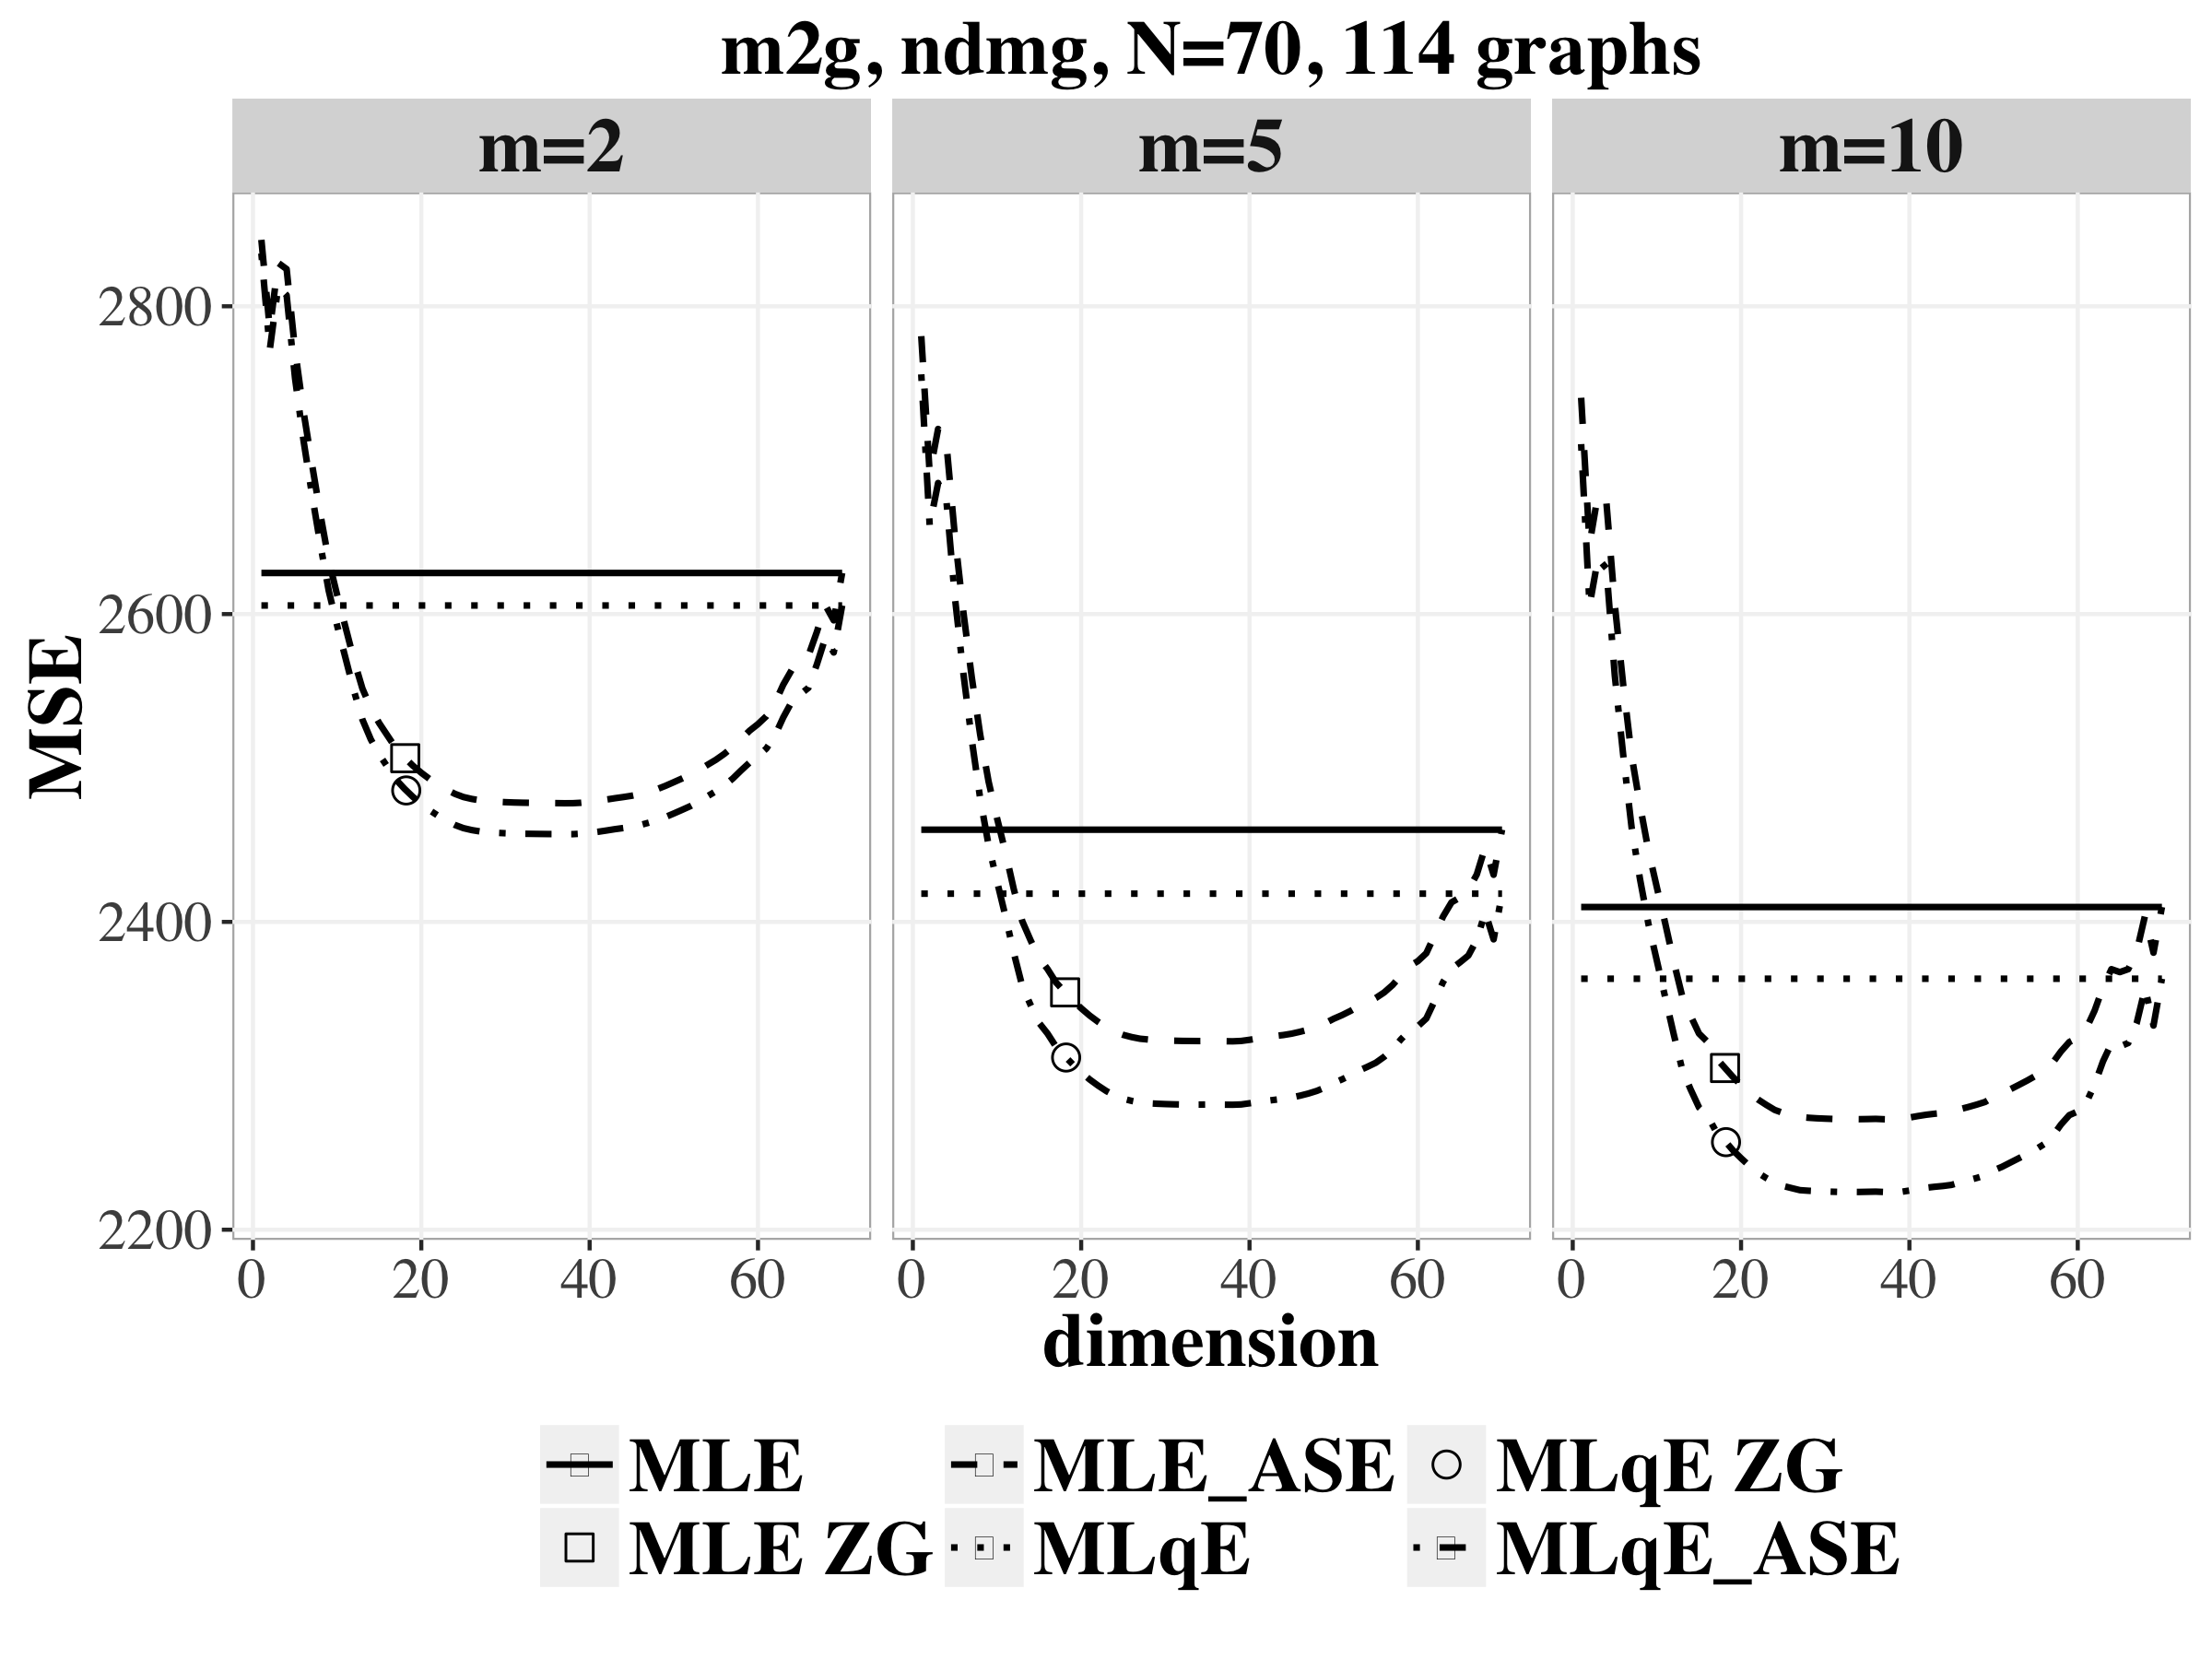
\includegraphics[width=\textwidth]{../../figs/CCI_m2g_ndmg_Weighted_q_0.9_EIG.png}
\caption{
{\bf Comparison of MSE of the four estimators for the desikan atlases at three sample sizes based on m2g and ndmg pipelines.}  
{\bf 1. MLE (horizontal solid line) vs MLqE (horizontal dotted line):} 
ML$q$E outperforms MLE since robust estimators are always preferred in practice;
{\bf 2. MLE (horizontal solid line) vs MLE\_ASE (dashed line):} MLE\_ASE wins the bias-variance tradeoff when embedded into a proper dimension; 
{\bf 3. MLqE (horizontal dotted line) vs ML$q$E\_ASE (dashed dotted line):}
ML$q$E\_ASE wins the bias-variance tradeoff when embedded into a proper dimension; 
{\bf 4.  ML$q$E\_ASE (dashed dotted line) vs MLE\_ASE (dashed
line):}
MLqE\_ASE is better, since it inherits the robustness from 
ML$q$E. And the square and circle represent the dimensions selected by the Zhu and Ghodsi method. We can see it does a pretty good job. But more importantly, a wide range of dimensions could lead to an improvement.
}
\label{fig:robDim}
\end{cframed}
\end{figure}


%% Feb
We had theorems for the ML$q$E under the exponential distribution. Actually the results can be generalized to a broader class of distribution families, and even a different entry-wise robust estimator other than ML$q$E with the following conditions:
\begin{compactenum}
\item Let $A_{ij} \stackrel{ind}{\sim} (1-\epsilon) f_{P_{ij}} + \epsilon f_{C_{ij}}$, then $E[(A_{ij} - E[\hat{P}_{ij}^{(1)}])^k] \le \mathrm{const} \cdot k!$, where $\hat{P}^{(1)}$ is the entry-wise MLE as defined before;
This is to ensure the that observations will not deviate from the expectation too far away, such that the concentration inequality can apply.
\item There exists $C_0(P_{ij}, \epsilon) > 0$ such that under the contaminated model with $C > C_0(P_{ij}, \epsilon)$,
\[
	\lim_{m \to \infty} \left| E[\hat{P}_{ij}] - P_{ij} \right| < 
    \lim_{m \to \infty} \left| E[\hat{P}^{(1)}_{ij}] - P_{ij} \right|;
\]\\
It requires the contamination of the model to be large enough (a restriction on the distribution) and $\hat{P}$ to be robust enough with respect to the contamination (a condition on the estimator).
\item $\hat{P}_{ij} \le \mathrm{const} \cdot \hat{P}_{ij}^{(1)}$; (This might be generalized to with high probability later)\\
Since we use the results of $\hat{P}^{(1)}$ to bound $\hat{P}^{(q)}$, the proof can apply directly with this condition for an arbitrary $\hat{P}$.
\item $\mathrm{Var}(\hat{P}_{ij}) = O(m^{-1})$, where $m$ is the number of observations.\\
We will get exactly the same results under this condition. However, even if the variance of the new estimator is not of order $O(m^{-1})$, we will get similar results with a different term related to $m$.
\end{compactenum}

\clearpage

%% March
Although we only present the results under exponential distributions, the results can be generalized to a broader class of distribution families, and even a different entry-wise robust estimator other than ML$q$E with the following conditions:
\begin{compactenum}
\item Let $A_{ij} \stackrel{ind}{\sim} (1-\epsilon) f_{P_{ij}} + \epsilon f_{C_{ij}}$, then $E[(A_{ij} - E[\hat{P}_{ij}^{(1)}])^k] \le \mathrm{const}^k \cdot k!$, where $\hat{P}^{(1)}$ is the entry-wise MLE as defined before;\\
This is to ensure that observations will not deviate from the expectation too far away, so that the concentration inequalities hold.
\item There exists $C_0(P_{ij}, \epsilon) > 0$ such that under the contaminated model with $C > C_0(P_{ij}, \epsilon)$,
\[
	\lim_{m \to \infty} \left| E[\hat{P}_{ij}] - P_{ij} \right| < 
    \lim_{m \to \infty} \left| E[\hat{P}^{(1)}_{ij}] - P_{ij} \right|;
\]\\
It requires the contamination of the model to be large enough (a restriction on the distribution) and $\hat{P}$ to be robust enough with respect to the contamination (a condition on the estimator).
\item $\hat{P}_{ij} \le \mathrm{const} \cdot \hat{P}_{ij}^{(1)}$;\\
Since we use the results of $\hat{P}^{(1)}$ to bound $\hat{P}^{(q)}$, the proof can apply directly with this condition for an arbitrary $\hat{P}$.
\item $\mathrm{Var}(\hat{P}_{ij}) = O(m^{-1})$, where $m$ is the number of observations.\\
We will get exactly the same results based on this order. However, even if the variance of the new estimator is not of order $O(m^{-1})$, we will get similar results with a different term related to $m$.
\end{compactenum}

Previously we consider the model to be based on exponential distribution, which is continuous and monotone. Now we consider Poisson distribution instead. Poisson distribution is a commonly used distribution for nonnegative graphs with integer values. And we will prove that it satisfies the conditions for generalization and as a result all theories apply directly.

Let $A_{ij} \stackrel{ind}{\sim} (1-\epsilon) f_{P_{ij}} + \epsilon f_{C_{ij}}$ with $f$ to be Poisson, then we proved that $E[(A_{ij} - E[\hat{P}_{ij}^{(1)}])^k] \le \mathrm{const}^k \cdot k!$, where $\hat{P}^{(1)}$ is the entry-wise MLE as defined before.
So Condition 1 is satisfied. Intuitively, since exponential distribution has a fatter tail compare to Poisson, we should have the bound for central moment of Poisson directly from the results for exponential distribution.
Condition 2 is satisfied as long as the contamination is large enough while keep using the robust ML$q$E.
For Condition 3, the extreme case happens when there are $m$ data $x_1, \cdots, x_m$ with $0 \le x_1 = \cdots = x_k \le \bar{x} \le x_{k+1} = \cdots = x_m \le m \bar{x}/(m - k)$. In order to have ML$q$E larger than MLE $\bar{x}$, we need the weights of the first $m$ data to be smaller than the weights of the rest $m - k$ data. So $e^{-\bar{x}} < \bar{x}^{x_m} e^{-\bar{x}} / x_m!$. Then $x_m! < \bar{x}^{x_m}$. By the lower bound in Stirling's formula, we have $x_m < e \bar{x}$ when $x_m > 0$. Note that if $x_m = 0$ then MLE equals ML$q$E since all data equals zero. Thus ML$q$E is bounded by $e \bar{x}$. As a result, $\hat{P}_{ij} \le e \hat{P}_{ij}^{(1)}$ and Condition 3 is satisfied.
At last, Condition 4 follows directly from theory of minimum contrast estimators.

So for all the theorems proved before, we can replace the exponential distribution by Poisson distribution and all the results still hold.

\clearpage
\end{document}
